\subsection{Two Peasants}

  \begin{figure}[h]
    \begin{center}
      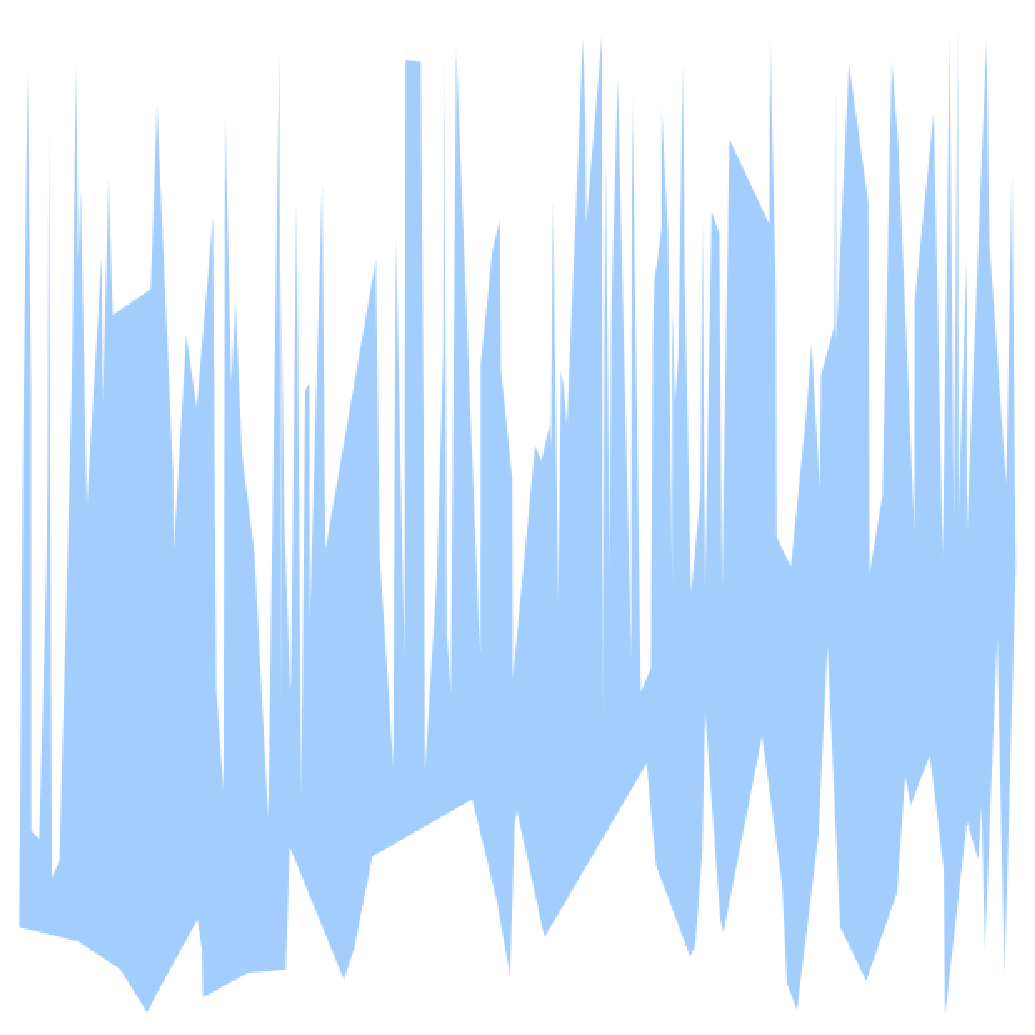
\includegraphics[width=0.3\textwidth]{img/twopeasants200.eps}
    \end{center}
    \caption{Polygon mit 200 Punkten (Two Peasants)}
    \label{fig:twopeasants200}
  \end{figure}

  \emph{Two Peasants} ist ein sehr einfacher Algorithmus ähnlich dem Algorithmus
  zur Erzeugung der konvexen Hülle einer Punktmenge, implementiert nach einer
  Beschreibung in~\cite{geometrylab}.

  \subsubsection{Algorithmus}

    Ausgehend von einer nach der $x$-Koordinate sortierten Punktmenge wird
    zunächst eine imaginäre Gerade zwischen den Extrempunkten gezogen.
    Oberhalb dieser Geraden werden anschließend die Punkte, die links der
    Geraden liegen, in Reihenfolge ihrer $x$-Koordinate verbunden.
    Anschließend werden die restlichen Punkte unterhalb der Geraden in
    umgekehrte Reihenfolge verbunden.

  \subsubsection{Eigenschaften}

  Der \emph{Two Peasants}-Algorithmus ermöglicht nicht die Erzeugung sämtlicher
  auf Grundlage einer Punktmenge denkbaren Polygone; er erzeugt im Gegenteil
  stets das selbe einfache Polygon. Die erzeugten Polygone lassen mit
  zunehmender Punktzahl deutlich die imaginäre Gerade zwischen den Extrempunkten
  erkennen. Oberhalb und unterhalb dieser Geraden entstehen zunehmend vertikale
  Strecken als Verbindung zwischen aufeinanderfolgenden Punkten der Punktmenge.
  Der Algorithmus ähnelt der natürlichen Vorgehensweise eines Menschen, der
  versucht aus einer gegebenen Punktmenge ein simples Polygon zu konstruieren
  (vgl.~\cite{geometrylab}). Die Laufzeit des Algorithmus wird dominiert von der
  Laufzeit des gewählten Sortieralgorithmus (bspw. im Normalfall $\bigO(n \log
  n)$), das Verbinden der sortierten Punkte zu einem Polygon erfolgt
  anschließend in linearer Zeit.
